\documentclass[a4paper,10pt,ngerman]{scrartcl}
\usepackage{babel}
\usepackage[T1]{fontenc}
\usepackage[utf8x]{inputenc}
\usepackage[a4paper,margin=2.5cm]{geometry}

% Die nächsten drei Felder bitte anpassen:
\newcommand{\Name}{BANDO} % Teamname oder eigenen Namen angeben
% \newcommand{\TeamId}{}
\newcommand{\Aufgabe}{Brainfire: Dokumentation}

% Kopf- und Fußzeilen
\usepackage{scrlayer-scrpage}
\setkomafont{pageheadfoot}{\textrm}
\ifoot{\Name}
\cfoot{\thepage}
\chead{\Aufgabe}
% \ofoot{Team-ID: \TeamId}

% Für mathematische Befehle und Symbole
\usepackage{amsmath}
\usepackage{amssymb}

% Für Bilder
\usepackage{graphicx}

% Für Algorithmen
\usepackage{algpseudocode}

% Für Quelltext
\usepackage{listings}
\usepackage{color}
\definecolor{mygreen}{rgb}{0,0.6,0}
\definecolor{mygray}{rgb}{0.5,0.5,0.5}
\definecolor{mymauve}{rgb}{0.58,0,0.82}
\lstset{
  keywordstyle=\color{blue},commentstyle=\color{mygreen},
  stringstyle=\color{mymauve},rulecolor=\color{black},
  basicstyle=\footnotesize\ttfamily,numberstyle=\tiny\color{mygray},
  captionpos=b, % sets the caption-position to bottom
  keepspaces=true, % keeps spaces in text
  numbers=left, numbersep=5pt, showspaces=false,showstringspaces=true,
  showtabs=false, stepnumber=2, tabsize=2, title=\lstname
}
\lstdefinelanguage{JavaScript}{ % JavaScript ist als einzige Sprache noch nicht vordefiniert
  keywords={break, case, catch, continue, debugger, default, delete, do, else, finally, for, function, if, in, instanceof, new, return, switch, this, throw, try, typeof, var, void, while, with},
  morecomment=[l]{//},
  morecomment=[s]{/*}{*/},
  morestring=[b]',
  morestring=[b]",
  sensitive=true
}

% Diese beiden Pakete müssen als letztes geladen werden
\usepackage{hyperref} % Anklickbare Links im Dokument
\usepackage{cleveref}

% Daten für die Titelseite
\title{\Aufgabe}
\author{\Name}
\date{\today}



\begin{document}
	
	\maketitle
	\tableofcontents
	
	
	\section{Pathfinder-Generierung}
		
		\subsection{Grundidee}
		
			Betrachte die zwei Punkt S (für "'Start"') und Z (für "'Ziel"') in einem Raum. Da der Raum in seiner Ausbreitung beschränkt ist, existieren von S zu Z - bei gewünschter Platzierung der Steine - auch nur eine endliche Anzahl an denkbarer Lösungspfade. Ein Algorithmus soll all diese Pfade bestimmen, sortieren und speichern. Die für einen Pfad notwendigen Steine sollen ebenfalls gespeichert werden, aber auch die Menge aller Felder, die nicht mit Steinen belegt werden dürfen.
			
			Wann immer ein Raum generiert werden soll, sodass mindestens eine Lösung von S nach Z existiert, so ist es hinreichend einen Pfad der gespeicherten Menge zufällig auszuwählen und die entsprechenden Felder mit Steinen zu belegen bzw. freizuhalten. Mögliche Laufzeit-Probleme sind auf diese Weise auf einen Zeitpunkt vor Beginn des Spiels verschoben worden. Das eigentliche Spiel bedarf auch nicht eines Algorithmus, der die Existenz einer Lösung sicherstellt.\\
			
			tl;dr: Die Eigenschaft, dass mindestens ein Lösungspfad von S nach Z in einem Raum existiert, wird durch eine zuvor untersuchte und langfristig gespeicherte Menge definiert.
		
		\subsection{Umsetzbarkeit}
		
			Um die Idee auf Umsetzbarkeit zu überprüfen, wurde ein Backtracking-Algorithmus geschrieben, der strukturiert alle Lösungspfade von S nach Z in einem beliebig großen Raum bestimmt. Obwohl die Punkte S und Z frei wählbar sind, wurden sie wie im Skript festgelegt: S ist ein Feld unter der links oberen Ecke und Z ist ein Feld über der rechts unteren Ecke.
			
			\begin{figure}[h!]
				\begin{center}
					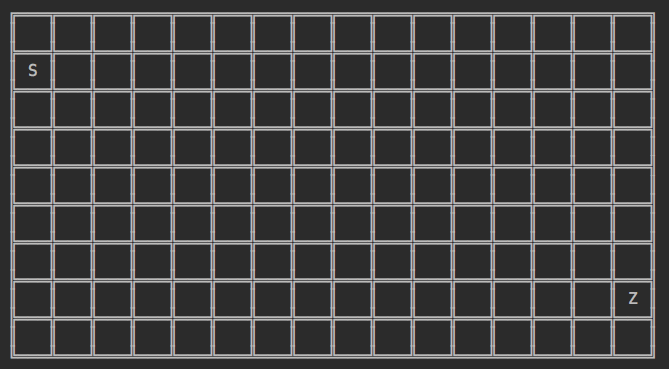
\includegraphics[width=1\textwidth]{SZ.png}
					\caption{Position von S und Z in einem 16 mal 9 Raum}
				\end{center}
			\end{figure}
			\newpage
			
			Der Algorithmus lieferte die Menge aller Lösungspfade und insbesondere auch die Anzahl der Lösungen. Folgende Tabelle hält die Menge aller Lösungen abhängig von der Dimension des Raums fest:
			
			\begin{figure}[h!]
				\begin{center}
					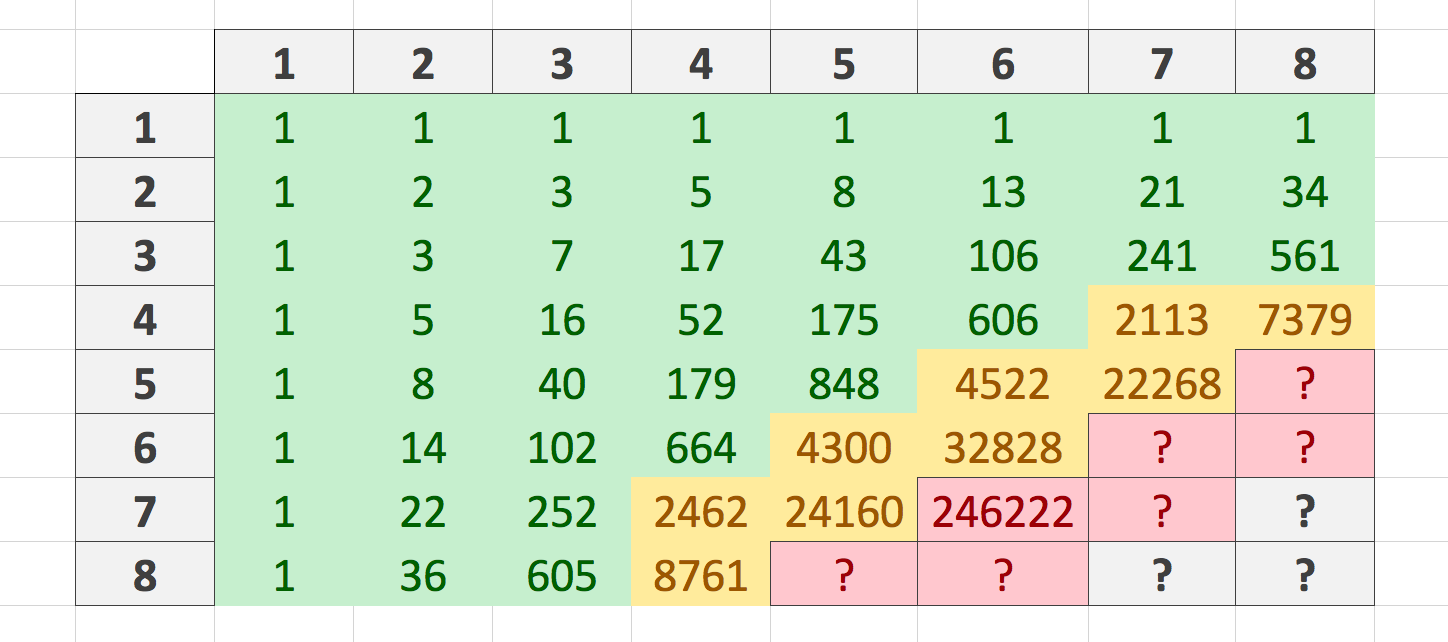
\includegraphics[width=1\textwidth]{Laufzeittabelle.png}
					\caption{Menge aller Lösungen in Abhängigkeit von Breite und Höhe des Raums}
				\end{center}
			\end{figure}
			
			Das Fazit, das aus dieser Betrachtung gezogen werden kann, ist, dass alle Raumgrößen im grauen Bereich der Tabelle nicht denkbar für diesen Generierungsansatz sind. Im besten Fall ist dieser Algorithmus für maximal 7x7 große Räume nutzbar.
		
		\newpage
		\subsection{Beispiel}
		
			\begin{figure}[h!]
				\begin{center}
					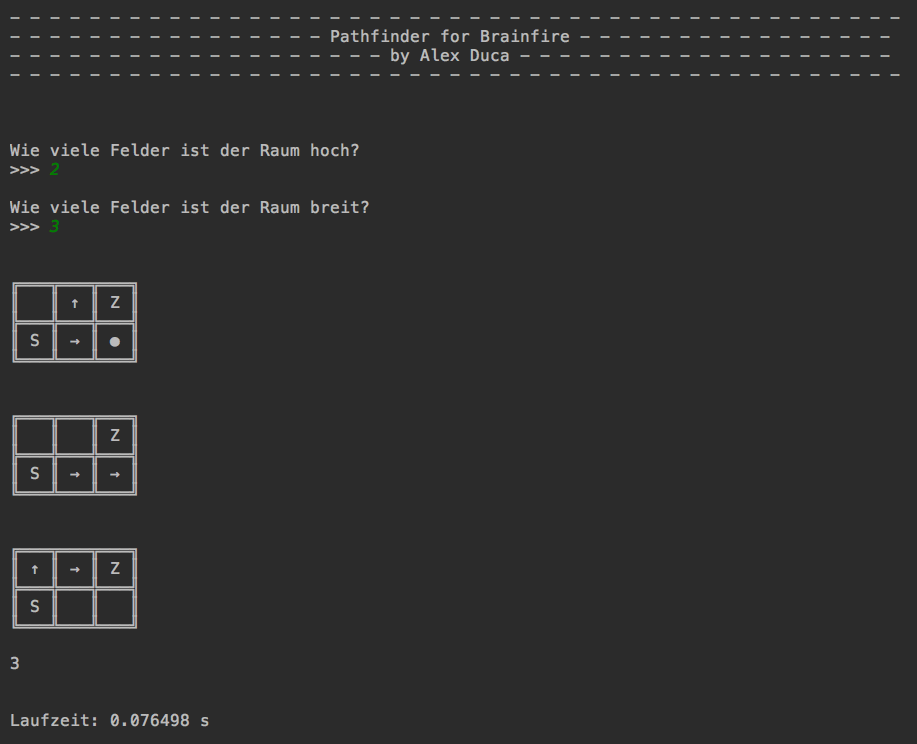
\includegraphics[width=1\textwidth]{2x3Beispiel.png}
					\caption{Menge aller Lösungen in einem 2x3-Raum}
				\end{center}
			\end{figure}





	\newpage
	\section{Spray 'n' Pray}
	
		\subsection{Grundidee}
		
			Im Vordergrund steht die Entwicklung eines sehr effizienten Algorithmus, der in kürzester Zeit bestimmt, von welcher Tür welche andere Tür erreicht werden kann. Das restliche Verfahren wird in zwei Teilschritte unterteilt:
			
			\begin{itemize}
				\item \textbf{Spray}: Es werden zufällig Steine auf dem Boden verteilt. Die Wahrscheinlichkeit, dass auf einer Fläche ein Stein liegt, wird im Folgenden bestimmt.
				\item \textbf{Pray}: Berechne mit dem Algorithmus die existenten Pfade und hoffe, dass der Raum brauchbar ist.
			\end{itemize}
	
			Auf diese Weise wird eine Riesenzahl \(N\) an Räumen erstellt und auf ihre Eigenschaften überprüft. Das daraus entstandene Repertoire an Räumen bildet die Auswahl für die Erstellung des Dungeons.


		\subsection{Umsetzung}

			Als Lösungsalgorithmus wird die Breitensuche verwendet, die über die Laufzeitkomplexität \(O(n^2)\) verfügt, wobei die Problemgröße \(n\) die Anzahl der Knoten in dem Suchbaum beschreibt. Da die Knoten durch die Felder des zu untersuchenden Raums bestimmt sind, hat der gesamte Lösungsalgorithmus eine Laufzeit von \( O( (a \cdot b)^2 ) \), wobei \(a,b\) die Seitenlängen des untersuchten Raums beschreiben. Bei einem quadratischen Raum der Seitenlänge \(n\) entspricht das Laufzeitverhalten also \( O(n^4) \). Im direkten Vergleich zum Backtracking-Algorithmus mit \( O(2^n) \) ist der Breitensuche-Algorithmus ein großer Erfolg.
			
			Mit Hilfe von Multiprocessing, ein Verfahren, das alle Computer-Kerne gleichzeitig belastet, lässt sich der Algorithmus zusätzlich um einen Linearfaktor beschleunigen.
			
		
		\subsection{Wahl der Parameter}

			Eine noch zu beantwortende Frage ist die Wahl des Parameters, der beschreibt, wie wahrscheinlich es ist, dass auf einem Feld ein Stein liegt: P(Stein). Mit Hilfe einer empirischen Untersuchung, die durch die folgende Tabelle festgehalten wurde, wird eine Antwort auf dieses Problem gegeben:
			
			\begin{figure}[h!]
				\begin{center}
					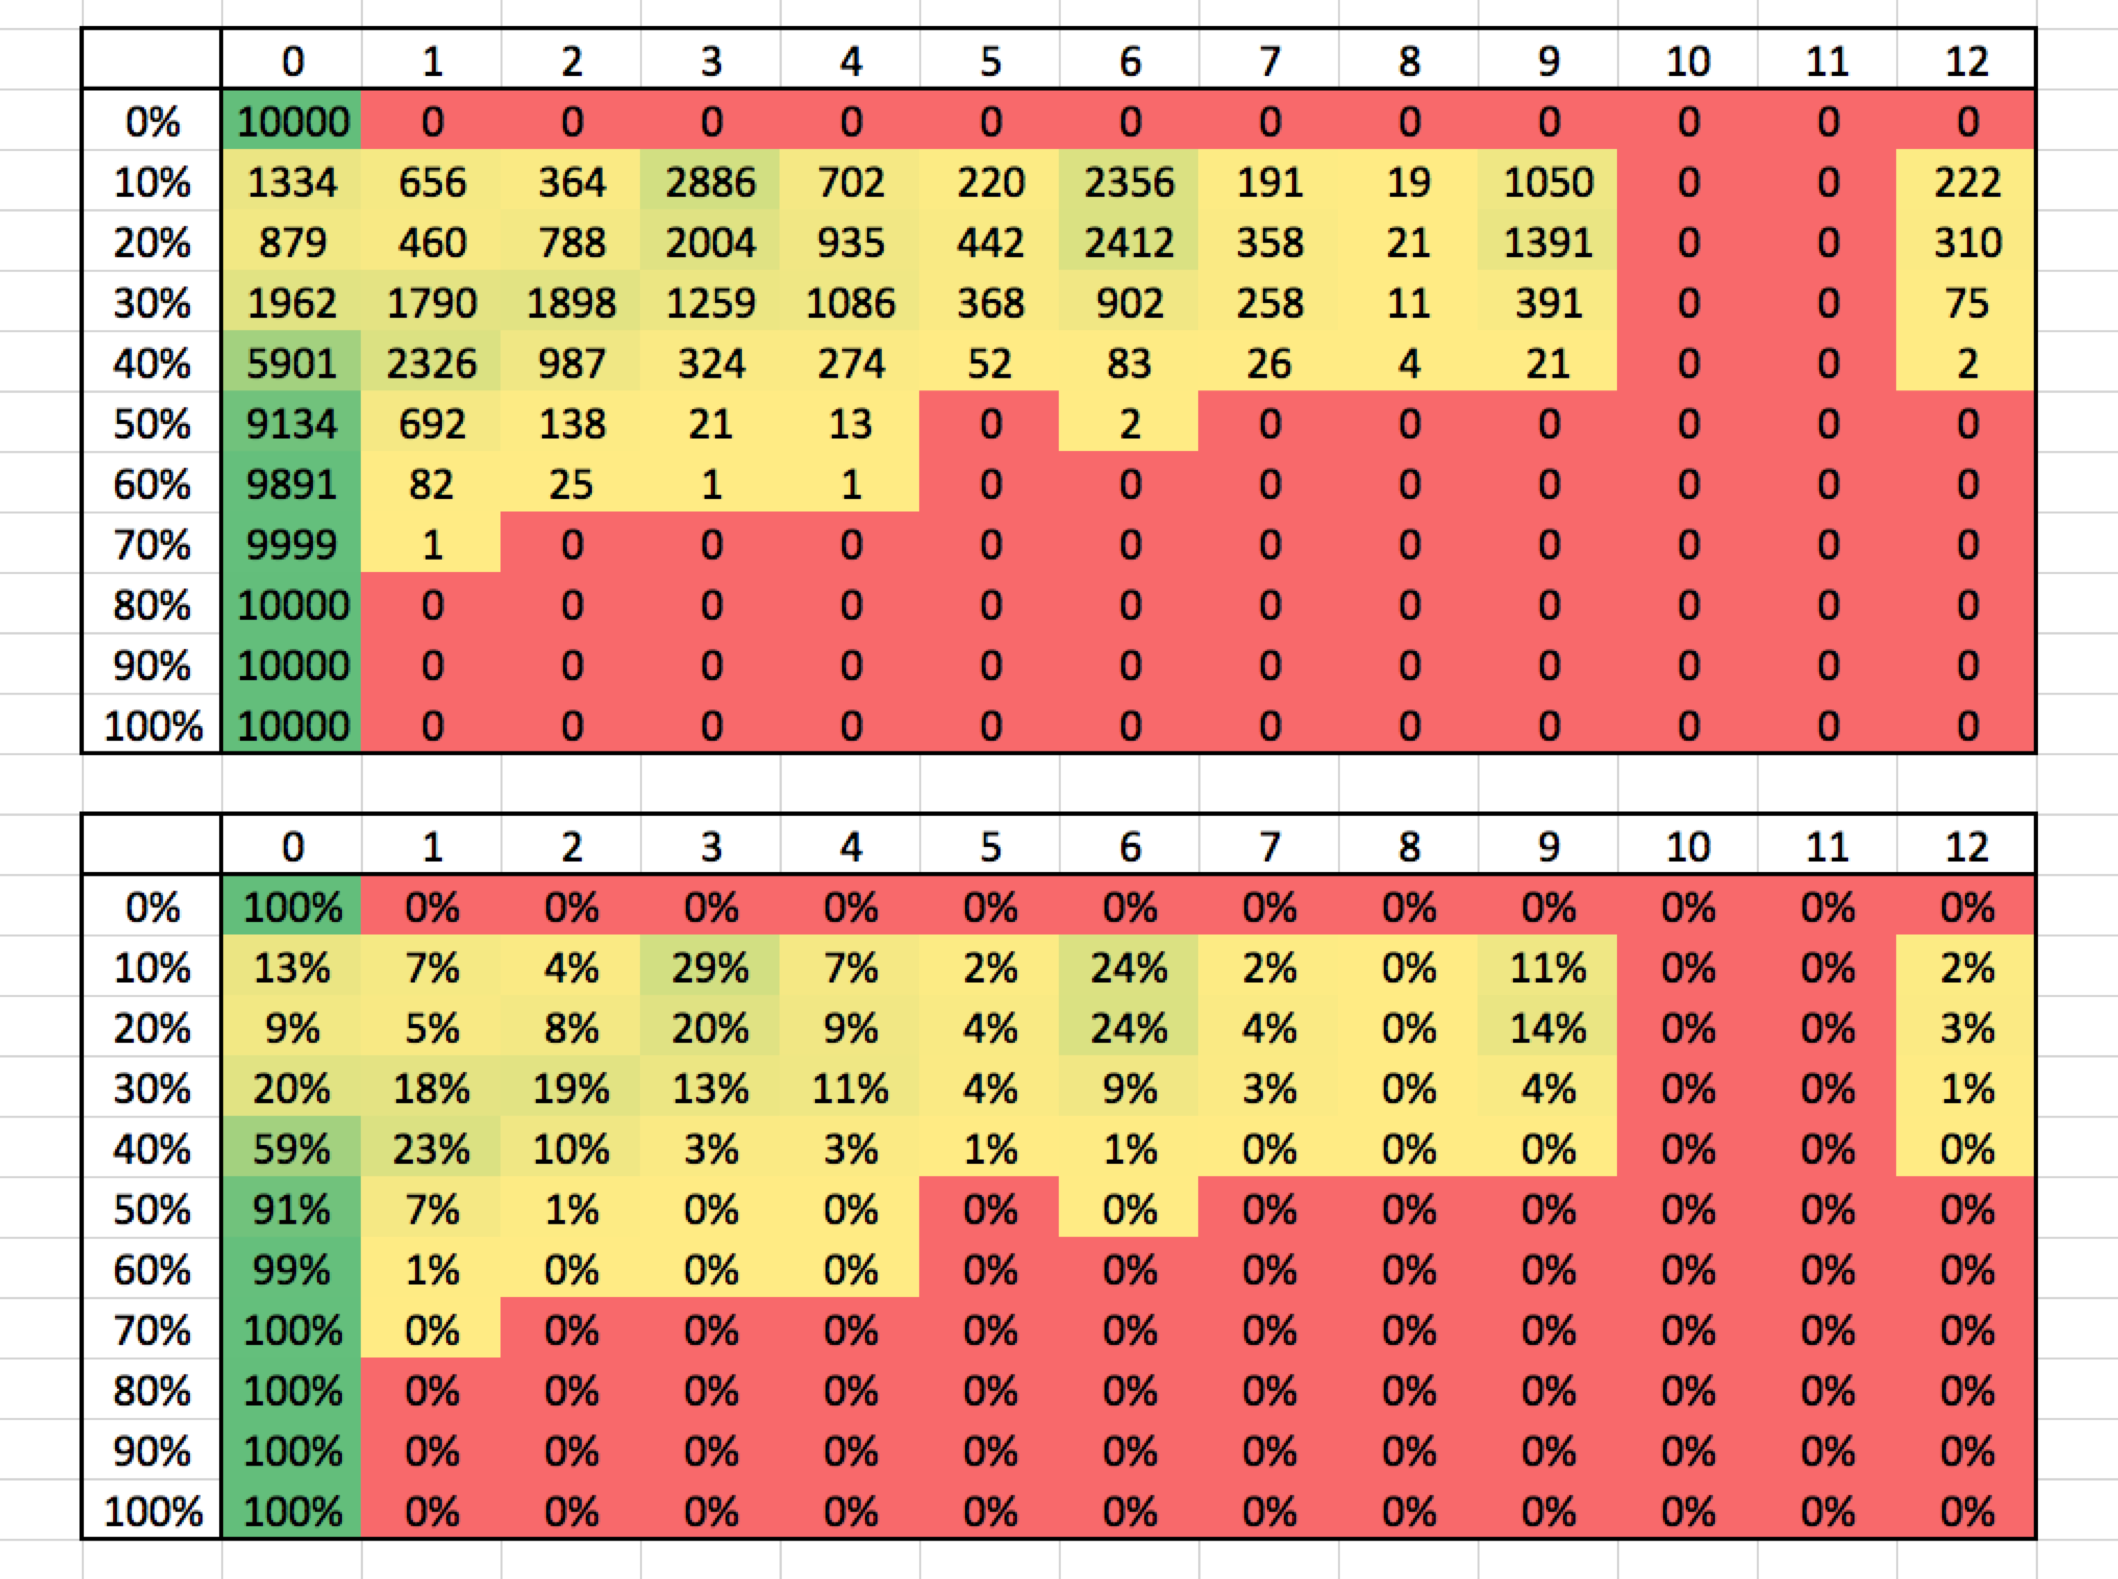
\includegraphics[width=0.75\textwidth]{pStein1.png}
					\caption{Betrachtet wird ein 16x16-Feld. Die y-Achse beschreibt P(Stein), die x-Achse beschreibt die Anzahl der Tür-Tupel (A,B), für die gilt, dass von Tür A aus Tür B erreichbar ist.}
				\end{center}
			\end{figure}
		
		\newpage


			Einen etwas detaillierteren Eindruck gibt die folgende Tabelle, die den Bereich  P(Stein) \( \in [12\%, 22\% ] \) betrachtet:
			
			\begin{figure}[h!]
				\begin{center}
					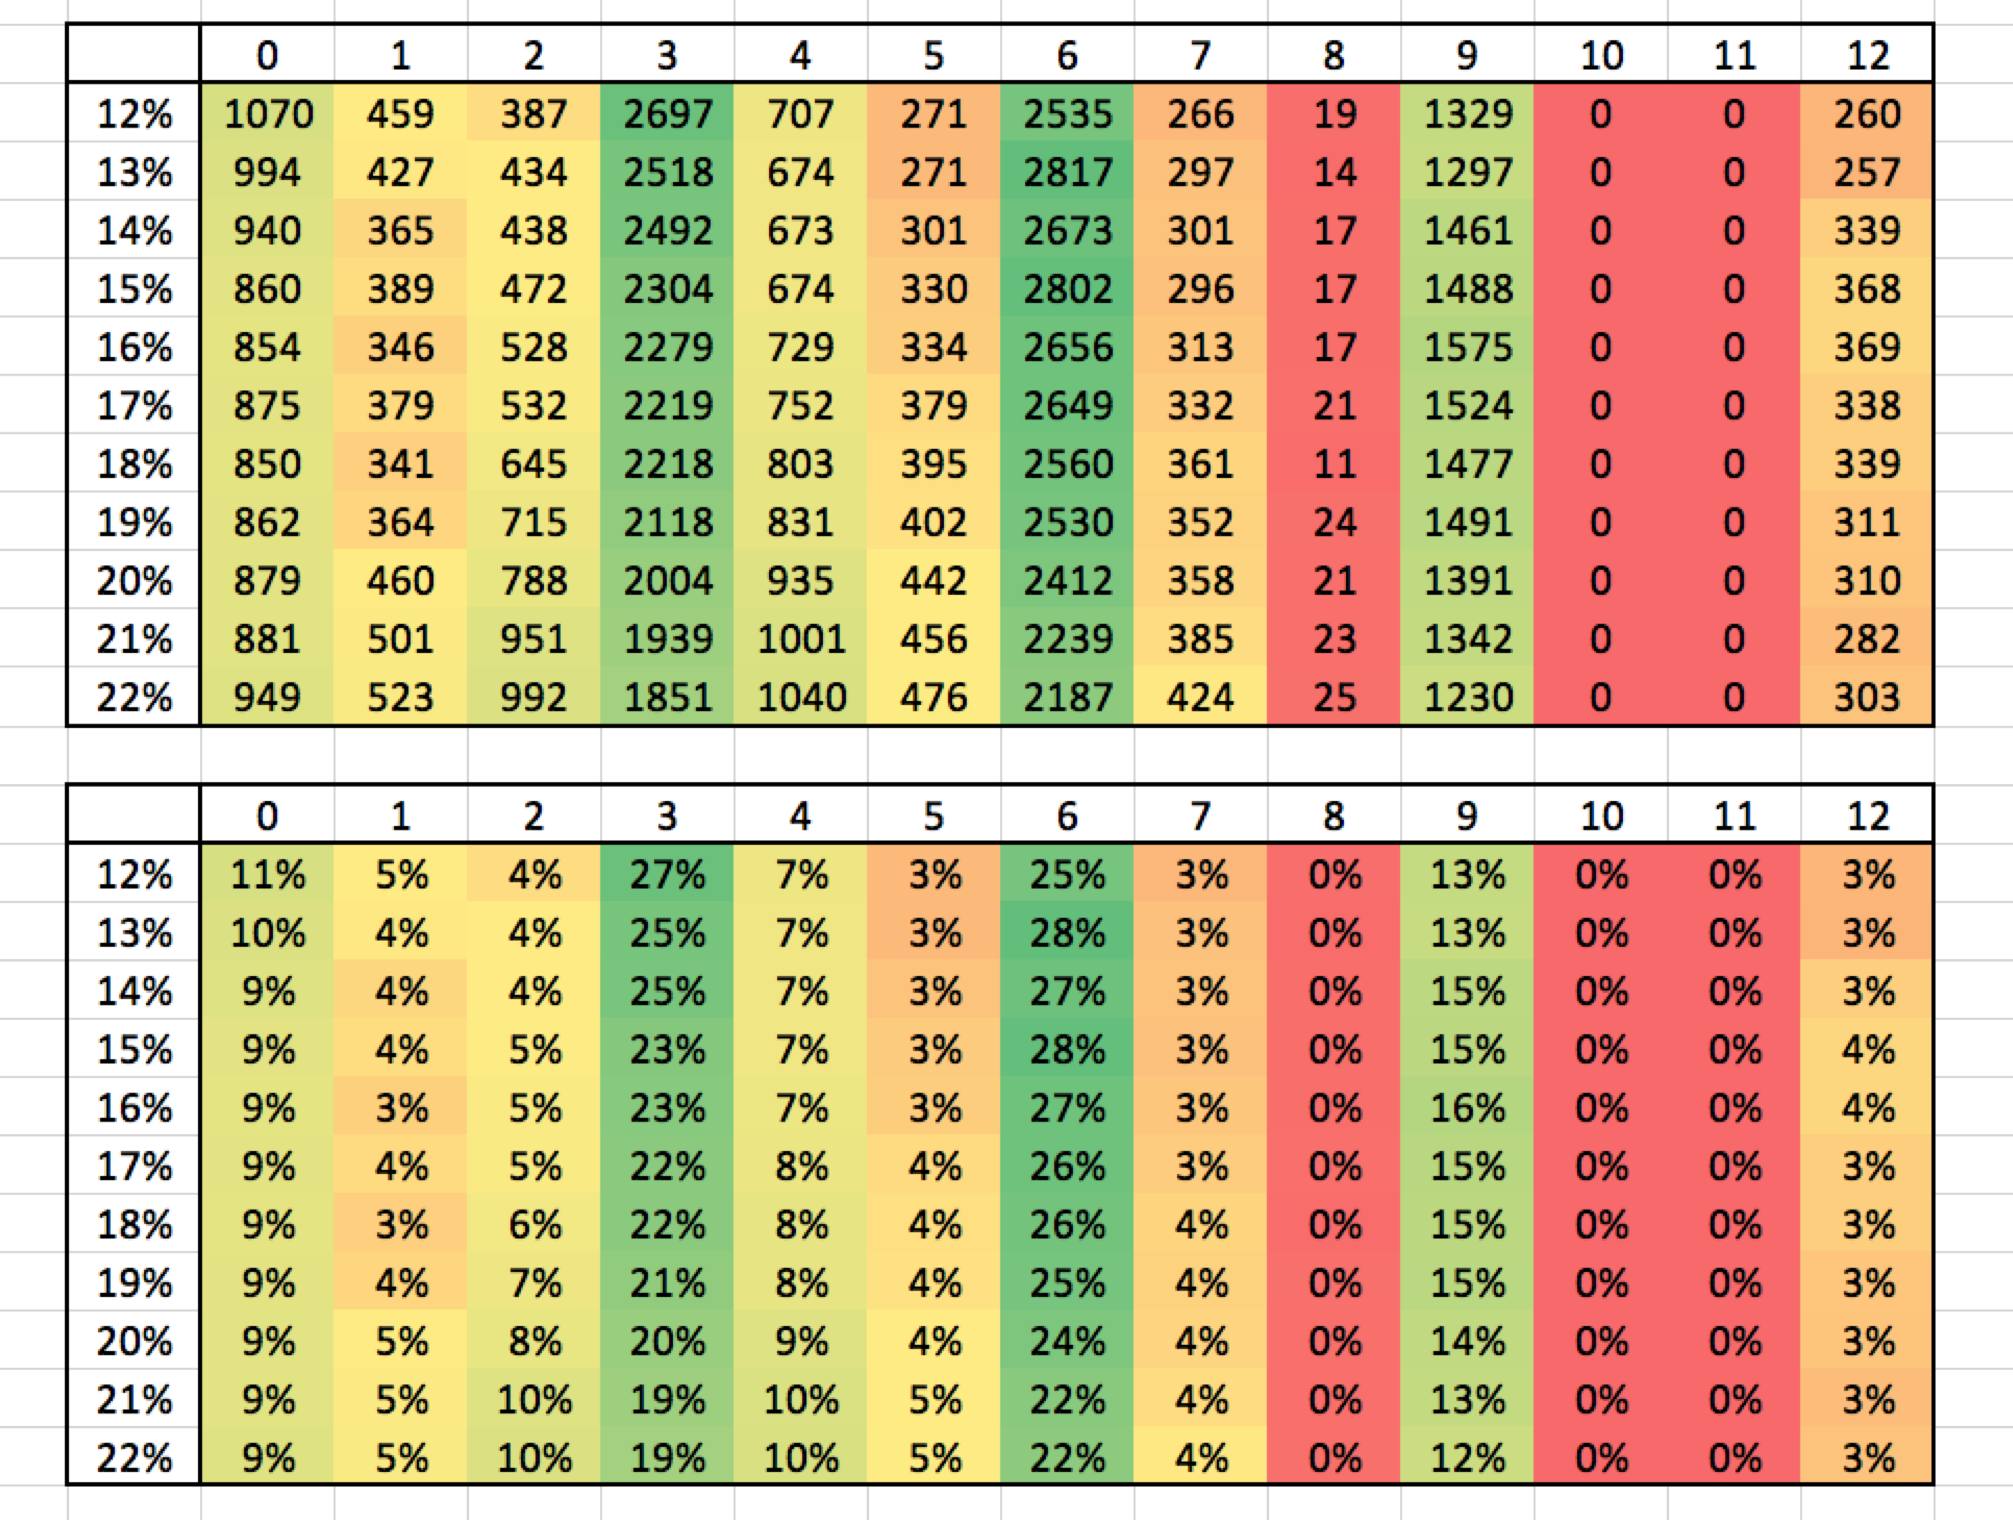
\includegraphics[width=0.75\textwidth]{pStein2.png}
					\caption{Betrachtet wird ein 16x16-Feld. Die y-Achse beschreibt P(Stein), die x-Achse beschreibt die Anzahl der Tür-Tupel (A,B), für die gilt, dass von Tür A aus Tür B erreichbar ist.}
				\end{center}
			\end{figure}
		
			Auf Grund der Homogenität dieses kleineren Suchbereichs lassen sich keine signifikante Aussagen über die ideale Wahl des Parameters P(Stein) machen. Der Durchschnittswert \( 18 \% \) ist gut geeignet, um die Wahrscheinlichkeit der Sackgassen-Räume (\( x  = 0 \)) möglichst zu minimieren.






	\newpage
	\section{Spray 'n' Pray: Dungeonlayout}
	
		\subsection{Grundidee}
		
			Aus den zuvor generierten und untersuchten Räumen wird eine zufällige Teilmenge gewählt und in einem Raster ausgelegt, sodass ein ganzer Dungeon entsteht. Als Ankerpunkte, die der Spieler der Reihe nach besucht, werden die Türen erachtet, die zwei aneinanderliegende Räume miteinander verbinden. Folgende Skizze veranschaulicht die Überlegung:
			
			\begin{figure}[h!]
				\begin{center}
					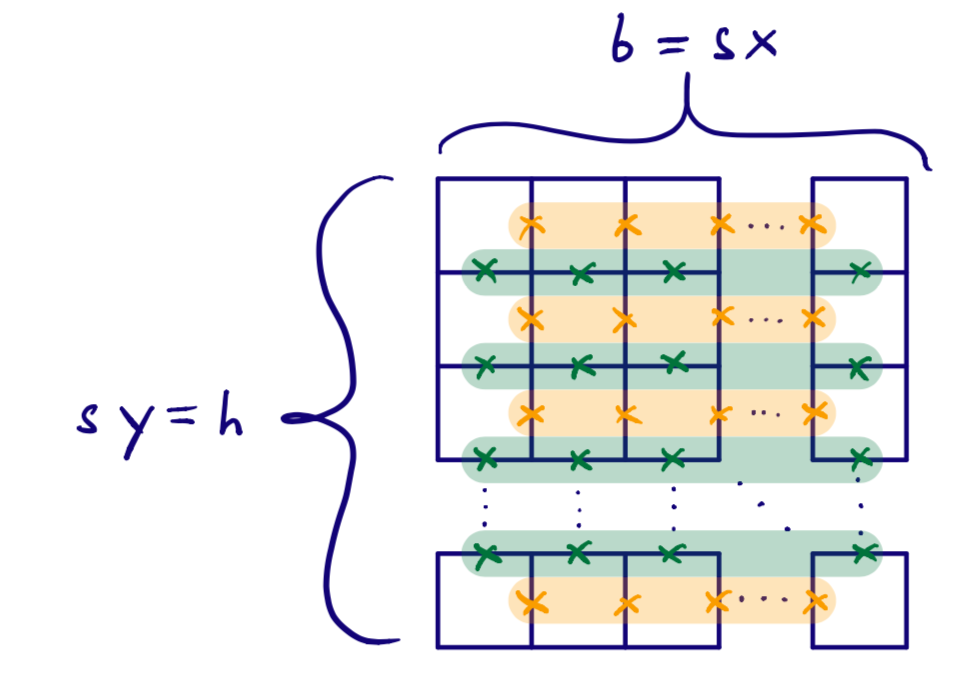
\includegraphics[width=0.5\textwidth]{tueren.png}
					\caption{Dungeon-Layout mit Breite \(b\) und Höhe \(h\). Die Kreuze stellen Türen dar.}
				\end{center}
			\end{figure}
			
			Relevant ist vor allem die Tatsache, dass der Spieler durch eine Ungeschickte Auswahl an Bewegungsfolgen in eine Sackgasse innerhalb eines Raums gelangen kann. Eine Reset-Funktion, die den Spieler zu der zuletzt besuchten Tür bringt, ist notwendig.
			
			Um also Sackgassen innerhalb des gesamten Dungeons zu verhindern und Lösbarkeit zu garantieren, müssen zwei Eigenschaften erfüllt sein:
			
			\begin{itemize}
				\item Die Starttür ist von jeder Tür aus erreichbar, die von der Starttür aus erreichbar ist. \\ (\textbf{"You Can Allways Go Home Again."})
				\item Die Endtür ist von der Starttür aus erreichbar. \\ (\textbf{"You Can Reach The Goal From Where You Start."})
			\end{itemize}
			
			Die Ausführung ist zuletzt analog wie im letzten Kapitel:
			
			\begin{itemize}
				\item \textbf{Spray}: Es werden zufällig Räume in einem Dungeon-Raster verteilt.
				\item \textbf{Pray}: Bestimme, ob die obigen Eigenschaften erfüllt sind.
			\end{itemize}
		
		\subsection{Umsetzung}
		
			Eine mathematische Funktion mit konstanter Laufzeit \( O(1) \) ist notwendig, um zu bestimmen, welche Räume sich welche Türen teilen. Der gesamte Dungeon wird dafür in ein Koordinatensystem getaucht, wobei die Ecke oben links die Koordinate \( (0,0) \) und die Ecke unten rechts die Koordinate \( (b,h) \) hat.
			
			Ein Raum, der in der Dungeon-Matrix die Koordinaten \( (x,y) \) hat, hat in dem Koordinatensystem den Raummittelpunkt \( (2x+1,2y+1) \). Alle Türen haben ebenfalls eine eindeutige Koordinate, die durch die Raummittelpunkte leicht erreichbar sind.
			
			
			

	\newpage
	\section{Gestaltung der Hintergrundmusik}
	
		\subsection{Inspirationsquellen}
		
			Da die Spielmechanik die Fortbewegung auf einer Eisfläche ist, soll Inspiration von Videospielmusikstücken gezogen werden, die ein Kälte-Motiv haben. Im Folgendem findet sich eine solche Auswahl.
			
			\subsubsection{The Legend of Zelda: Ocarina of Time}
			
				"'Ice Cavern"' (\href{https://youtube.com/watch?v=bcXuwXKsqMY}{bit.ly/2L22Kf2}) ist eine Eishöhle, in der Link unter anderem riesige Blöcke über einem Eisboden rutschen lässt, um eine Treppe zu seinem Ziel zu bauen. (\href{https://youtube.com/watch?v=uaGb3PtSPDg}{bit.ly/2LbnzDH})
			
			
			\subsubsection{The Legend of Zelda: Majora's Mask}
			
				"'Snowhead Temple"' (\href{https://youtube.com/watch?v=uxPDVDpbskI}{bit.ly/2Uc8sOl}) ist ein hoher zugefrorener Turm, zu dessen Spitze Link navigieren muss. In der Mitte des Turms findet sich eine Säule, dessen Höhe anpasst werden muss, indem von Goronen-Link vereinzelte Eisschichten aus der Säule raus geschlagen werden. (\href{https://youtube.com/watch?v=yM8440G32gk}{bit.ly/2Zx7Xj5})
			
			
			\subsubsection{Pokemon HeartGold/SoulSilver}
			
				"'Ice Path"' (\href{https://youtube.com/watch?v=riClBdyycM4}{bit.ly/2HwBQtH}) ist eine Eishöhle, die mit jener Spielmechanik arbeitet, von der dieses ganze Projekt inspiriert wurde. (\href{https://youtube.com/watch?v=erqrS-e-piA}{bit.ly/30EPnqp})
	
	
			\subsubsection{Super Mario Galaxy}
			
			"'Ice Mountain"' (\href{https://youtube.com/watch?v=9qnJWbEnKOs}{bit.ly/348siys}) ist ein Musikstück, das in der "'Freezeflame Galaxy"' gespielt wird. Das Spiel führt zu diesem Zeitpunkt eine Bewegungsmechanik ein, mit der Mario über Eis Schlittschuh fahren kann. Auch findet sich in dieser Welt das Power-Up "'Iceflower"', die Mario für eine begrenzte Zeit die Fähigkeit gibt, Wasseroberflächen einzufrieren, um zusammen mit der Bewegungsmechanik zum Ziel zu navigieren. (\href{https://youtube.com/watch?v=ImsaYCFMJns}{bit.ly/2zt42sN})
		

\end{document}
